\section{Implementation}
%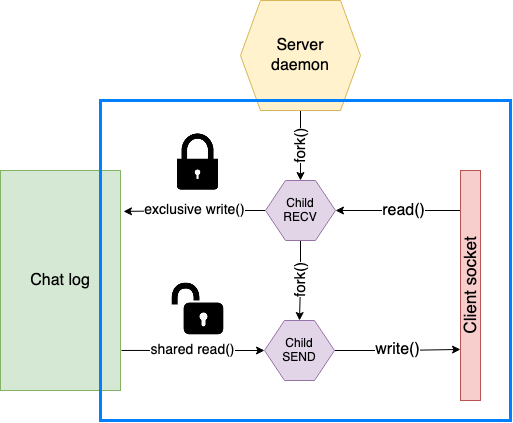
\includegraphics[width=1in,height=1.25in,keepaspectratio]{img/server.png}
\begin{figure}[!t]
	\centering
	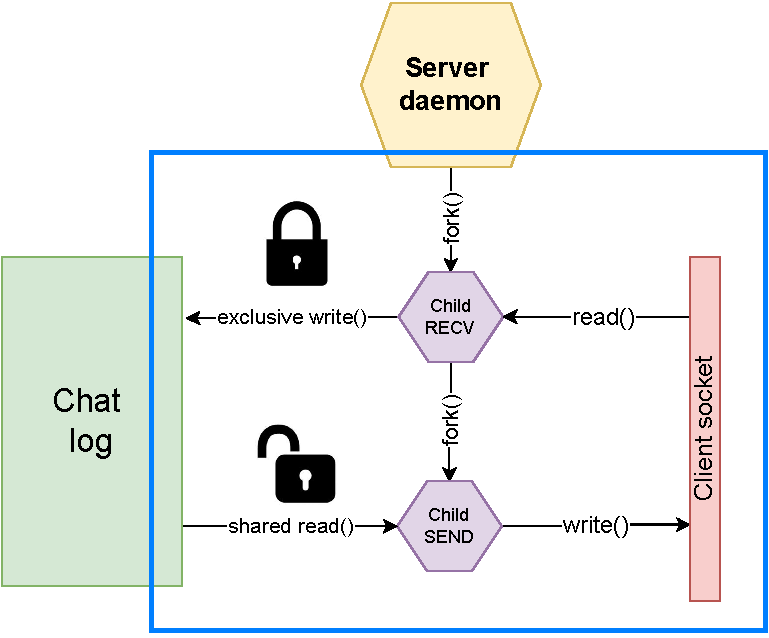
\includegraphics[width=2.5in]{img/server.pdf}
	%where an .eps filename suffix will be assumed under latex, 
	%and a .pdf suffix will be assumed for pdflatex; or what has been declared
	%via \DeclareGraphicsExtensions.
	\caption{Server's back-end process overview}
	\label{fig_server_backend}
\end{figure}
The requirements for the chat application are that an undefined number of participants can simultaneously exchange text messages in a chatroom. Furthermore, the communication might be asynchronous, so that the participants can read messages sent to them while they were not connected to the server. To ease portability across Unix systems, the application should use the least amount of dependencies as possible.

The server fundamentally requires a process working as a daemon accepting incoming connection attempts from clients. For each accepted client connection there are multiple possibilities regarding server architecture. The daemon could handle each client separately in a unique thread or child process.

The server will mostly have an IO-bound workload, consisting of handling asynchronous network packets and writing the messages from the users into files in the server's filesystem. An IO-bound workload benefits from the use of a pre-emptive scheduler, since the threads or processes are constantly changing alternatively from a blocked and an unblocked state in an unpredictable manner. As soon as a client goes silent the pre-emptive scheduler can run any other runnable process \cite{Kennedy2018}. Hence, the context-switching is actually advantageous for IO-bound workloads, whereas in CPU-bound workloads (e.g. intensive long-running sequential computations) it becomes a performance bottleneck.

Therefore, handling each client connection separately by forking a child process seems like a good fit for the kind of workload that is expected. Nonetheless, it must be acknowledged that a counterargument against using processes from a performance stand point is that thread creation and context-switching times are generally faster than for processes, since processes have an inherently more complex memory layout than threads \cite{Kerrisk2010}.

However, two other reasons settled the decision towards processes instead of threads. First, compartmentalizing the different clients into separate processes has some  



--------------------------------------

Mention that there were also portability issues, and that a different behaviour between the development environment and the production or deployment environment was seen. A system call was been compiled differently (the default flags were being used, which where different between systems) so working entirely with gcc and the the standard C library is not a guaranty for automatic perfect portability. In fact, it was very cumbersome to debug the faulty behaviour, since it had to be done using strace, in order to find the misbehaving syscall. Conclusion, thinking that using only C, gcc and the stdlib is working almost dependency-free is a fallacy or an illusion, debugging unexplained behaviour will still be arduous.